\section{Evaluation}


\section{Evaluation strategy}

\subsection{Experiment setup}

\subsection{User study}
Users are to be divided into two groups at random. One group of users will be asked to drive around the track without having any feedback provided by the system. This will evaluate how much a user can improve on their own. While the second group will also be asked to drive around, but this time the system will provide feedback on where and how the user can improve. A set of questions will be asked to the user once the test is complete. The questioner is meant to collect data on the users' racing experience prior to taking the test. Telemetry data will also be collected for both groups. Statistical analysis will be carried to determine if lap times do improve. 

\subsection{Sample Demographic}

\subsection{Data Analysis}

\begin{figure}[!htb]
	\centering
	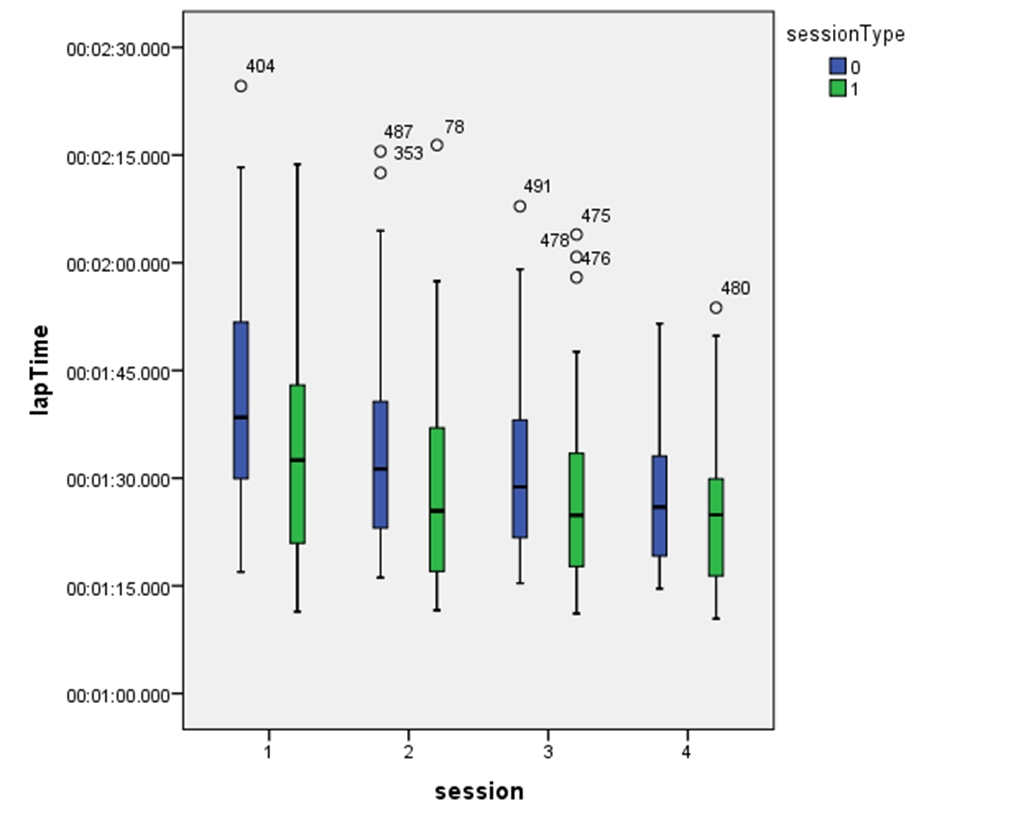
\includegraphics[height=7cm]{images/LapTimes}
	\caption{Lap Times}
	\label{fig:LapTimes}
\end{figure}

\begin{figure}[!htb]
	\centering
	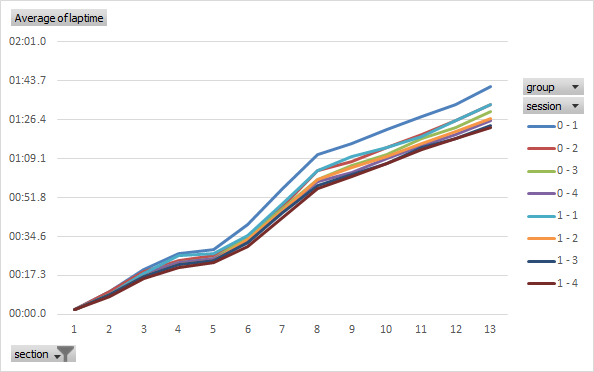
\includegraphics[height=7cm]{images/LapSections}
	\caption{Lap Sections}
	\label{fig:LapSections}
\end{figure}

\begin{figure}[!htb]
	\centering
	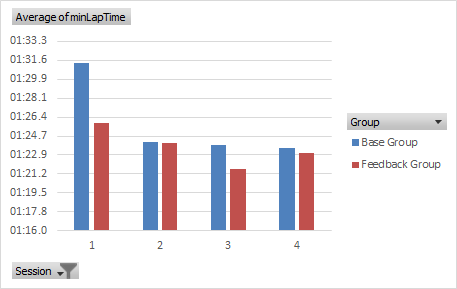
\includegraphics[height=7cm]{images/LapMinCompare}
	\caption{Lap Min Compare}
	\label{fig:LapMinCompare}
\end{figure}